\documentclass[10pt]{article}
\usepackage[margin=16mm]{geometry}
\usepackage{graphicx,booktabs,hyperref}
\usepackage[strings]{underscore}
\setlength{\parindent}{0pt}\setlength{\parskip}{4pt}
\begin{document}
\section*{Quartic IC: four-rung native replay}
Completed native smoke and independent replay, 2026-10-25.
Session \texttt{ECBS1h3b825b093913}: 24 records,
24 verified, 24/24 deterministic replays identical,
zero audit problems. Every native audit check passes. This completes this
four-rung correctness smoke, not the larger crossover campaign.

Base-field m=6,8,10,12, seed 1, max cofactor 16; two independently generated
public one-target workloads per rung. Arms: bin-t-line / gaudry-d4-bin with
Frobenius-reduced equations, same-point negation rho, and identical rho repeat.
One round, no warmup, alternate order, 900-second native child limit, L0.
The arbitrary coefficients include b outside the quadratic subfield;
proper extension structure used by IC does not make q-Frobenius an
automorphism of this same curve. Exact ICV1 identities:

{\footnotesize \path{ICV1:f2m-24-b060917d:1171:16776046:0x5712a5:unk:unk:r:7fbf6d93de36}\\
\path{ICV1:f2m-32-62005e2d:-45925:4295013222:0x26c0d997:unk:unk:r:abb49a5ab5c9}\\
\path{ICV1:f2m-40-1d6ebc58:573363:1099511054414:0xf11e9533ce:unk:unk:r:49958dc16466}\\
\path{ICV1:f2m-48-254ef1ce:-17036033:281474993746690:0x8875f7c10c02:unk:unk:r:cfcd93896112}}

\begin{center}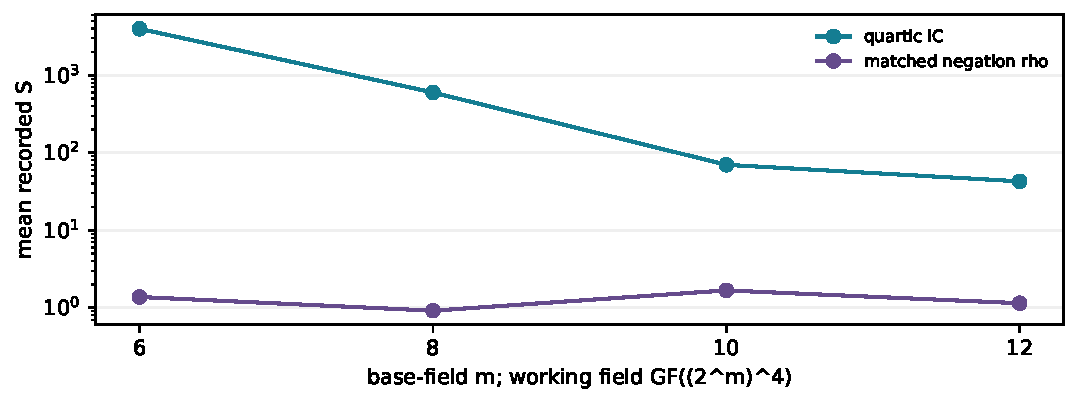
\includegraphics[width=.98\linewidth]{quartic-smoke-costs.pdf}\end{center}
\begin{center}\begin{tabular}{rrrr}\toprule
Base m & subgroup r & IC S, mean of 2 & rho S, mean of 2\\\midrule
6 & 1198289 & 3978.13 & 1.375765 \\
8 & 715835537 & 599.8988 & 0.9154702 \\
10 & 549755527207 & 69.89538 & 1.67309 \\
12 & 28147499374669 & 42.75407 & 1.142728 \\
\bottomrule\end{tabular}\end{center}

Unit: recorded GAE / square root of r, using the adapter's deterministic
Fq-operation conversion and seeded lift probes. These count conventions
are not nanoseconds or measured hardware prices. Raw IC costs independently
reconstruct from integer counts. The canonical band refuses missing global
calibration rows; its exact refusal and separately labeled compatibility
and all-native scenarios are in the pricing audit. Word scans, physical
conversion and other complete-cost obligations remain unresolved. Two targets
give no population interval. No measured crossover or complete-price win is
inferred; historical m=14 and extrapolated crossover claims remain separate.

Spec, plan, host and sealed rows: \path{../../pipeline-runs/quartic-smoke-20261025-02/}.
Independent replay: \path{../../pipeline-receipts/quartic-smoke-20261025-02.json}.
Pricing: \path{../run-pricing-audit-20261025/report.pdf}.
Source: src/cryptanalysis/gaudry_quartic_bin.rs and native ecbench adapters.
m=14/15 full panels remain outstanding; m=16--18 need wider arithmetic.
The separate HKY continuation retains its memory failures. No leaderboard
or admitted benchmark row is promoted.

\end{document}
